


\renewcommand{\title}{Certificat de spécialisation analyste de données massives (STA211)}
% -> author name and surname
\renewcommand{\author}{Boukary OUEDRAOGO}
\renewcommand{\abstract}{Avec l'explosion des données de ces dernières années, le besoin de tirer de la valeur des grands gissements de données est de plus en plus d'actualité. Les recherches théoriques qui restaient jadis dans les centre de recherche ont eu un regain d'intérêt grâce notamment au évolutions technologiques dans les domaines de l'informatique. Ces évolutions technologiques ont rendu possible le stockage et le traitement des données de grandes dimensions. Ces données opérationnelles qui sont optimisées pour le stockage et pas pour le traitement nécessité une certaine ingénierie pour permettent aux entreprises de tirer de la valeur de celles-ci.
}

\begin{titlepage}
\thispagestyle{empty}

\begin{tikzpicture}[remember picture,overlay]
\node at (current page.south west)
{\begin{tikzpicture}[remember picture, overlay]
  \shade[bottom color=bubblegum,top color=white] (0,0) rectangle
  (\paperwidth,.7\paperheight);
  \node [color=gray!50,rotate=-20]at (0.35\textwidth,9){\resizebox{7cm}{1.5cm}{$\displaystyle \ln\left(\frac{P}{1-P}\right) = \beta_0 + \sum_{p=1}^{P} \beta_{p}X_p   $}};
  
   \node [rotate=-0.5]at (0.7\textwidth,13){\resizebox{12cm}{7cm}{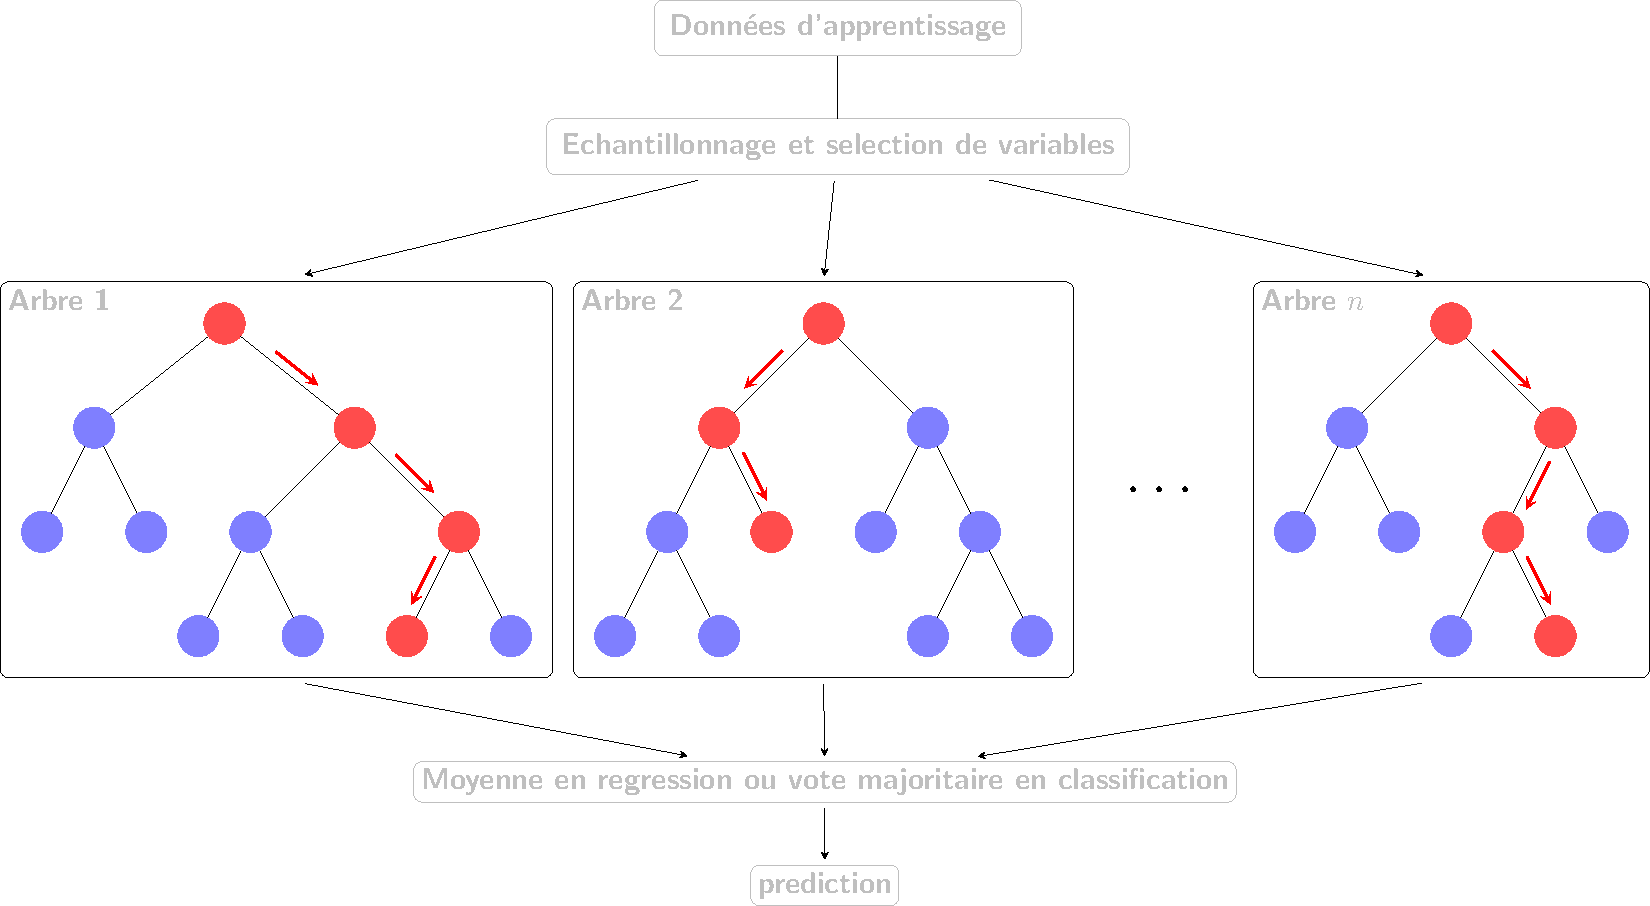
\includegraphics[]{include/random-forest.pdf}}};
  
  
  \node [color=gray!50,rotate=-5]at (.6\textwidth,4){\resizebox{9cm}{5cm}{\def\layersep{2.5cm}

\begin{tikzpicture}[shorten >=1pt,->,draw=black!50, node distance=\layersep]
    \tikzstyle{every pin edge}=[<-,shorten <=1pt]
    \tikzstyle{neuron}=[circle,fill=black!25,minimum size=17pt,inner sep=0pt]
    \tikzstyle{input neuron}=[neuron, fill=green!50];
    \tikzstyle{output neuron}=[neuron, fill=red!50];
    \tikzstyle{hidden neuron}=[neuron, fill=blue!50];
    \tikzstyle{annot} = [text width=4em, text centered]

    % Draw the input layer nodes
    \foreach \name / \y in {1,...,4}
    % This is the same as writing \foreach \name / \y in {1/1,2/2,3/3,4/4}
        \node[input neuron, pin=left:Input \#\y] (I-\name) at (0,-\y) {};

    % Draw the hidden layer nodes
    \foreach \name / \y in {1,...,5}
        \path[yshift=0.5cm]
            node[hidden neuron] (H-\name) at (\layersep,-\y cm) {};

    % Draw the output layer node
    \node[output neuron,pin={[pin edge={->}]right:Output}, right of=H-3] (O) {};

    % Connect every node in the input layer with every node in the
    % hidden layer.
    \foreach \source in {1,...,4}
        \foreach \dest in {1,...,5}
            \path (I-\source) edge (H-\dest);

    % Connect every node in the hidden layer with the output layer
    \foreach \source in {1,...,5}
        \path (H-\source) edge (O);

    % Annotate the layers
    \node[annot,above of=H-1, node distance=1cm] (hl) {Hidden layer};
    \node[annot,left of=hl] {Input layer};
    \node[annot,right of=hl] {Output layer};
\end{tikzpicture}}
  };
  
  \node [color=gray!50,rotate= 30]at (1\textwidth,8){\resizebox{7cm}{1.5cm}{{\Large MSE}$\displaystyle= \frac{1}{n}\sum_{i=1}^{n} \left(Y_i -\hat{Y}_{i }\right)^2$}};
  \end{tikzpicture}
};

\end{tikzpicture}


\vspace{-1cm}
%-----------------------------------------------------------------------------------
  %  page de garde
%-----------------------------------------------------------------------------------
  \begin{center}

\begin{large}

\includegraphics[width=8cm, height=3.5cm]{Images/le_cnam.png} \\
\textsc{Certificat de spécialisation analyste de données massives}\\ \bigskip
\textbf{ Entreposage et fouille de données
} \end{large}
\end{center}
\bigskip
\shadowoffset{3pt}
\begin{tcolorbox}[blanker,top=1.2cm,bottom=1.2cm,borderline horizontal={4pt}{0pt}{bluePoli},colupper=bluePoli]
\begin{center}
\shadowtext{\resizebox{\textwidth}{1.cm}{{\small Synthèse du cours }}}
\end{center}
\end{tcolorbox}


\bigskip

\begin{minipage}{0.4\textwidth}
\large
\emph{Réalisé par:}\\
\author\\[3mm]
\end{minipage}\\[2cm] 


%\textcolor{bluePoli}{\rule{.82\textwidth}{4pt}\hfill {\fontfamily{pzc}\fontsize{.7cm}{0cm}\selectfont \YEAR }}
\end{titlepage}


\AddToShipoutPicture*{\BackgroundPic}
\small \normalfont

\vspace{11pt}

\centerline{\rule{1.0\textwidth}{0.4pt}}

\begin{center}
\begin{minipage}[t]{.24\textwidth}
\begin{minipage}{.90\textwidth}
\noindent
\scriptsize{\textbf{Professeur:}} \\
\advisor \\
\\
\textbf{Année académique:} \\
\YEAR \\
\\
\end{minipage}
\end{minipage}% This must go next to `\end{minipage}`
\begin{minipage}{.74\textwidth}
\noindent \textbf{\color{bluePoli} Résumé:} {\abstract}
\end{minipage}
\end{center}

\vspace{15pt}

\begin{tcolorbox}[arc=0pt, boxrule=0pt, colback=bluePoli!60, width=\textwidth, colupper=white]
    \textbf{Mots-clés:} \keywords
\end{tcolorbox}

\vspace{12pt}

